\documentclass[numbers=noenddot, openany]{thesis}

% hier namen etc. einsetzen
\fullname{Lukas Hennig\\Felix Rottler\\Natalie Spister}
\headline{Advanced Mobile Business Applications\\Dokumentation}
\jahr{2018}
\gutachterA{Marc Schickler}
\typ{Anwendungsfach }
\fakultaet{Ingenieurwissenschaften, Informatik und \\Psychologie}
\institut{Institut für Datenbanken und Informationssysteme}

\hypersetup{%
	pdftitle=\pdfescapestring{\thetitel},
	pdfauthor={\thefullname},
 	pdfsubject={\thetyp},
}

\usepackage{graphicx}
\usepackage{caption}
\usepackage{subcaption}
\usepackage{float}
\usepackage{wrapfig}
\usepackage{lipsum}

% trennungsregeln
\hyphenation{Sil-ben-trenn-ung}

\begin{document}
\frontmatter
\maketitle
% impressum
\impressum

% ab hier zeilenabstand 1,4 fach 10pt/14pt
\setstretch{1.4}

\section*{Kurzfassung}
Im Rahmen der Veranstaltung Advanced Mobile Application Engineering 

Die Kurzfassung (engl. Abstract) einer Abschlussarbeit enthält zwei Blöcke. Der
erste Block enthält eine  kurze Hinführung/Motivation zum Thema sowie einer
anschließenden Beschreibung der Problemstellung (ca. 5-8 Sätze). Der zweite
Block der Kursfassung gibt die Zielsetzung bzw. den Beitrag der Abschlussarbeit
wieder (ebenfalls ca. 5-8 Sätze).

===========================================

ChangeLog:

2015-10-12: Hacks für Literaturverzeichnis eingebaut. Kommentare in der BibTex
Datei beachten!

2015-07-21: Fakultätname angepasst (+ Psychologie)




% inhaltsverzeichnis einfügen
\tableofcontents

\mainmatter
% hier kommen die kapitel der arbeit
% % %
%
%	- Einleitung- 
%
%	Ziel:	Gib eine schöne Einleitung mit Motivation, Problemstellung, Zielsetzung und Struktur der Arbeit
%
%	Status: alpha
%
% % %
\chapter{Einleitung}
\label{cha:einleitung}
Hier kommt die Einleitung mit Motivation hin.

% Abschnitt: Problemstellung
\section{Problemstellung}
\label{sec:einleitung:problemstellung}
Beschreibe in diesem Abschnitt die Problemstellung der Arbeit!

% Abschnitt: Zielsetzung
\section{Zielsetzung}
\label{sec:einleitung:zielsetzung}
Beschreibe in diesem Abschnitt die Zielsetzung der Arbeit!

% Abschnitt: Struktur der Arbeit
\section{Struktur der Arbeit}
\label{sec:einleitung:struktur}
Beschreibe in diesem Abschnitt die Struktur der Arbeit!

\chapter{Grundlagen}
\label{cha:grundlagen}
In diesem Abschnitt werden kurz einige Grundlagen, die für das Spiel wichtig sind, erklärt. 

%Abschnitt: Jump 'n' Run
\section{Jump 'n' Run (Platformer)}
\label{sec:grundlagen:jumpnrun}
Die Anwendung soll das vorhandene Spielprinzip des Jump 'n' Runs übernehmen und eigene Ideen einfließen lassen. Wie der Name schon suggeriert zeichnet sich ein Jump 'n' Run - Spiel dadurch aus, dass die Spielfigur durch \textit{springen} und \textit{laufen} Hindernisse überwinden und in den meisten Fällen ein Ziel erreichen muss. Zusätzlich kann dem Spieler die Möglichkeit gegeben werden zu \textit{schießen}, zu \textit{klettern} oder zu \textit{kämpfen}. \\
Das klassiche Jump 'n' Run ist in 2D und die Spielfigur läuft von links nach rechts, wobei der Fokus der Kamera stets auf der gesteuerten Spielfigur liegt. 


%Abschnitt: Multiplayer
\section{Multiplayer}
\label{sec:grundlagen:multiplayer}
Klassische Jump'n'Run Spiele wie Mario sind für Einzelspieler konzipiert, aber schon mit der ersten Playstation \cite{playstation} setzten sich Multiplayerspiele durch, zunächst waren aufgrund der begrenzten Controller nur zwei Spieler möglich. Kabellose Controller und der Durchbruch des Internets eröffneten jedoch die Möglichkeit einer nahezu unbegrenzten Anzahl von Spielern ein gemeinsames Spielerlebnis. \\
Um dies zu ermöglichen wird auf einer mobilen Platform eine Verbindung zu einem Server, also damit ein Server und eine bestehende Internetverbindung benötigt. Die Spiellogik selber wird über ein Netzwerk realisiert, ein Beispiel für solch ein Netzwerk sind die \textit{Google Play Services} \cite{googleplayservices} von Google. In Unity gibt es dafür das \textit{Photon Unity Networking}, welches in Kapitel \ref{subsec:realisierung:technologien:photon} genauer betrachtet wird.


% Abschnitt: Spielgrundlagen
\section{Spielablauf}
\label{sec:grundlagen:spielgrundlagen}
Abyss soll ein levelbasiertes Jump'n'Run Multiplayer Spiel werden. \newline
Ganz wie andere Platformer sollen die Spieler sich auf Plattformen in eine Richtung bewegen. Da das Spiel levelbasiert sein soll, ist das Ziel des Spielers das Ende eines jeden Levels zu erreichen und ins nächste Level zu gelangen. \\
Um Eintönigkeit beim Spiel zu vermeiden werden die Level mit unterschiedlichen Schwierigkeiten implementiert, dabei sollen nicht nur Spielitems wie z.B. Power-Ups zum Einsatz kommen, sondern auch bewegliche Objekte, die dem Spieler auch Schaden hinzufügen können. \\
Damit der Spieler sich möglichst gut im Spiel zurechtfindet wird die Steuerung minimal und möglichst einfach gehalten, so können auch Fehleingaben vermieden werden. Des Weiteren soll das Spiel nur im Multiplayermodus gespielt werden können, also werden immer zwei Spieler benötigt um das Spiel zu starten. 
% Steuerung Anfoderung

\chapter{Anforderungen}
\label{cha:anforderungen}
In diesem Kapitel werden die Anforderungen an das Spiel definiert. Dabei legen die funktionalen Anforderungen fest, wozu das Spiel imstande sein soll. Die nicht-funktionalen Anforderungen beschreiben, wie gut diese Anforderungen umgesetzt werden sollen.

% Abschnitt: Funktionale Anforderungen
\section{Funktionale Anforderungen}
\label{sec:grundlagen:funktionaleAnforderungen}
In Tabelle \ref{tab:grundlagen:funktionaleAnforderungen} werden die funktionalen Anforderungen an das Spiel und die jeweilige Priorisierung mit Werten von 1 (unwichtig) bis 5 (unabdingbar) formuliert.

\begin{center}
    \label{tab:grundlagen:funktionaleAnforderungen}
    \begin{tabular}{ c | l | c}
        Abkürzung & Anforderung & Priorität\\
        \hline
        FA01 & An- und Abmelden & 4 \\
        \hline
        FA02 & Spiel erstellen & 5 \\
        \hline
        FA03 & Spiel beitreten & 5 \\
        \hline
        FA04 & Multiplayer (2 Spieler) & 5 \\
        \hline
        FA05 & Animation der Spieler & 4 \\
        \hline
        FA06 & Verschiedene Level & 4 \\
        \hline
        FA07 & Verschiedene Level-Themen & 3 \\
        \hline
        FA08 & Verschiedene Spielobjekte & 4 \\
        \hline
        FA09 & Animation der Spielobjekte & 2 \\
        \hline
        FA10 & Simple Spielsteuerung & 5 \\
    \end{tabular}
    \captionof{table}{Funktionale Anforderungen} 
\end{center}

\textbf{FA01 An- und Abmelden}\\*
Der Nutzer kann sich im Spiel anmelden. Anschließend kann er das Spiel uneingeschränkt verwenden. Er bleibt so lange angemeldet bis er sich abmeldet.

\textbf{FA02 Spiel erstellen}\\*
Ein Spiel kann von jedem angemeldeten Nutzer erstellt werden. Dabei kann der Nutzer nur die Level verwenden, die er freigeschalten hat.

\textbf{FA03 Spiel beitreten}\\*
Jeder Nutzer kann jedem beliebigen Spiel beitreten unabhängig davon welche Level der Nutzer selbst freigeschalten hat.

\textbf{FA04 Multiplayer}\\*
Das Spiel soll ausschließlich von zwei Nutzern gespielt werden können. Die Nutzer sollen dabei den jeweiligen Mitspieler auf ihrem eigenen Gerät sehen können. Zudem soll teilweise ein kooperatives Spiel zwischen den Spielern erzwingbar sein.

\textbf{FA05 Animation der Spieler}\\*
Die verschiedenen Möglichkeiten der Steuerung eines Spielers sollen mit Animationen unterlegt werden. 

\textbf{FA06 Verschiedene Level}\\*
Es soll mehr als ein Level geben. Der Nutzer hat anfangs nur die Möglichkeit das erste Level zu spielen. Erst nach Abschluss eines Levels wird das nächste freigeschalten.

\textbf{FA07 Verschiedene Level-Themen}\\*
Die Level sollen sich im Design voneinander unterscheiden. Die Spielerfiguren und Spielobjekte bleiben dabei die gleichen im Aussehen und in ihrer Funktion.

\textbf{FA08 Verschiedene Spielobjekte}\\*
Durch verschiedene Spielobjekte innherhalb des Spiels wird das Spiel abwechslungsreich und komplex. Jedes dieser Spielobjekte hat dabei einen unterschiedlichen Effekt.

\textbf{FA09 Animation der Spielobjekte}\\*
Die Spielobjekte sollen durch Animationen als solche hervorgehoben werden. Dabei können sie bei Aktivierung verschiedene Effekte/Animationen/Geräusche machen, die den Zweck des Spielobjekts entprechen.

\textbf{FA10 Simple Spielsteuerung}\\*
Das Spiel soll möglichst einfach gesteuert werden können, d.h. auch das Eingaben, die möglicherweise falsch interpretiert werden können (Wischen in verschiedene Richtungen oder langes Drücken), sollen möglichst vermieden werden.


% Abschnitt: Nicht-Funktionale Anforderungen
\section{Nicht-Funktionale Anforderungen}
\label{sec:grundlagen:nichtFunktionaleAnforderungen}
Die in Kapitel \ref{sec:grundlagen:funktionaleAnforderungen} beschriebenen funktionale Anforderungen bestimmen die Funktionen und Umfang des Spiels. In der Tabelle \ref{tab:grundlagen:nichtFunktionaleAnforderungen} werden nun die nichtfunktionalen Anforderungen dargelegt, die die Qualität der Umsetzung festlegen.

\begin{center}
    \label{tab:grundlagen:nichtFunktionaleAnforderungen}
    \begin{tabular}{ c | l | c}
        Abkürzung & Anforderung & Priorität\\
        \hline
        NFA01 & Zuverlässigkeit & 5 \\
        \hline
        NFA02 & Aussehen und Handhabung & 5 \\
        \hline
        NFA03 & Benutzbarkeit & 4 \\
        \hline
        NFA04 & Funktionalität & 5 \\
        \hline
        NFA05 & Effizienz & 3 \\
    \end{tabular}
    \captionof{table}{Nichtfunktionale Anforderungen} 
\end{center}

\textbf{NFA01 Zuverlässigkeit}\\*
Das Spiel ist konsistent in der Ausführung. Es bricht nicht unerwartet ab und jedes Level kann von beiden Spielern beendet werden.

\textbf{NFA02 Aussehen und Handhabung}\\*
Das Spiel hinterlässt einen einen guten optischen Eindruck und besitzt eine uintuitive Steuerung.

\textbf{NFA03 Benutzbarkeit}\\*
Der Ablauf des Spiels ist leicht ersichtlich, sowohl im Menü als auch in den jeweiligen Level.

\textbf{NFA04 Funktionalität}\\*
Die in Kapitel \ref{sec:grundlagen:funktionaleAnforderungen} vorgestellten Anforderungen werden abhängig von ihrer Priorisierung erfolgreich umgesetzt.

\textbf{NFA05 Effizienz}\\*
Das Spiel soll auf dem eigenen als auch auf dem Gerät des Mitspielers flüssig laufen. 




\chapter{Konzeption \& Entwurf}
\label{cha:konzeption}
In diesem Kapitel wird das anfängliche Spielkonzept mit Hilfe von Mock-Ups visualisiert und evaluiert. Anschließend wird in Kapitel \ref{sec:konzeption:konzept} das umgesetzte Spielkonzept vorgestellt.

\section{Mock-Ups}
\label{sec:konzeption:prototyping:mockups}
Die ursprüngliche Idee des Spiels war ein Spielverlauf von oben nach unten, wodurch die beiden Spieler einen Abgrund (\textit{Abyss}) hinabspringen müssen, um einen Endgegner zu bekämpfen. Dabei springen beide Spieler durchgehend und um mit der Device-Motion die Richtung zu ändern (ähnlich zu \href{https://play.google.com/store/apps/details?id=com.lima.doodlejump&hl=de}{\textit{Doodle Jump}}). Jedoch sind durch dieses Leveldesign die Möglichkeiten der Levelgestaltung, als auch die Bewegungsfreiheit der Spieler stark eingeschränkt.
\begin{figure}[H]
    \begin{center}
      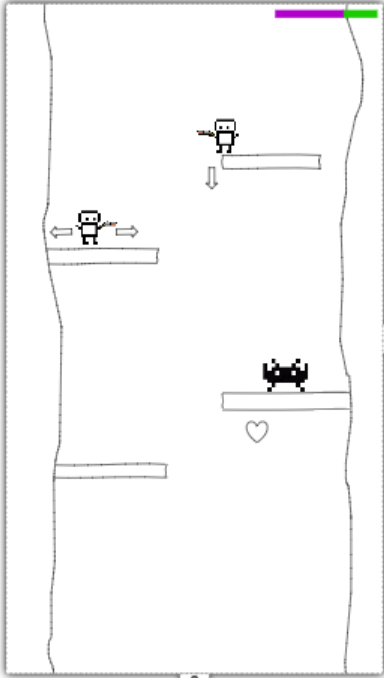
\includegraphics[width=.22\linewidth]{img/konzeption/Jump}
      \caption{Steuerung}
      \label{fig:konzeption:prototyping:jump}
    \end{center}
\end{figure}


Zusätzlich sollten Waffen in dem Spiel eingesetzt werden können, jedoch sind die Steuerungsmöglichkeiten an einem Smartphone mit den Möglichkeiten zu springen, schießen und bewegen des Spielers stark eingeschränkt und fehleranfällig.

\begin{figure}[H]
    \begin{center}
      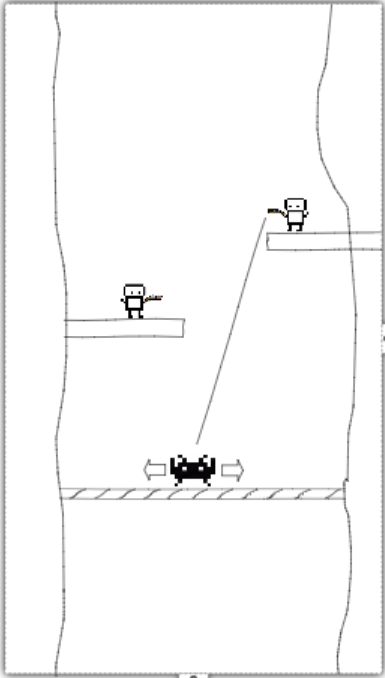
\includegraphics[width=.22\linewidth]{img/konzepFtion/Fight}
      \caption{Waffen}
      \label{fig:konzeption:prototyping:fight}
    \end{center}
\end{figure}


Zur Beendigung des Levels müssen beide Spieler das Ende erreichen um anschließend einen Endgegner zu besiegen. Wie in Kapitel \ref{sec:implementierung:probleme} erklärt, ist das designen von Assets anspruchsvoll und zeitaufwendig.
\begin{figure}[H]
    \begin{center}
      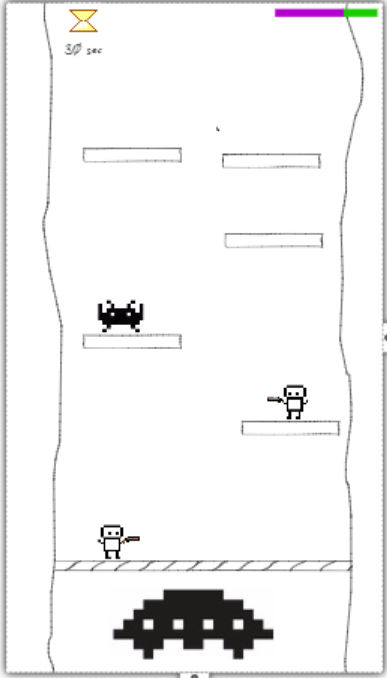
\includegraphics[width=.22\linewidth]{img/konzeption/EndBoss}
      \caption{Endboss}
      \label{fig:konzeption:prototyping:endboss}
    \end{center}
\end{figure}

\section{Spielkonzept}
\label{sec:konzeption:konzept}
In diesem Kapitel werden Spieleigenschaften, der Aufbau der Level und der Funktionsumfang der verschiedenen Spielobjekte erläutert. Die Ansicht der Spiels ist zweidimensional, daher werden die Level stets von der Seite dargestellt.

\subsection{Level}
\label{sec:konzeption:konzept:level}
 Die jeweiligen Level des Spiels beschäftigen sich mit einem eigenen Thema (mit eigenem Licht, Musik und Umfeld). Um ein Zusammenspielen der Spieler zu erzwingen müssen beide Spieler das Level beenden. Erst wenn beide Spieler das Ziel erreichen, ist das Level beendet. Damit das Level beendet werden kann, müssen im Laufe des Spiels zwei Schlüssel eingesammelt, die es erst ermöglichen das Ziel in Form einer Truhe zu erreichen. Spieler können anfangs nur das erste Level spielen, erst nach Beendigung des Levels wird das darauffolgende Level freigeschalten und somit spielbar. 

\subsection{Spielobjekte}
\label{sec:konzeption:konzept:spielobjekte}
Um das Spiel für den Spieler attraktiver zu gestalten werden verschiedene Spielobjekte verwendet, die das Spiel interessanter und abwechslungsreicher gestalten sollen. Diese Spielobjekte können den Spieler einen Vorteil verschaffen (\textit{Power-Up}), Schaden zufügen (\textit{Gegner}) oder transportieren (\textit{Plattform}). Zusätzlich gibt es Spielobjekte, die das Passieren eines bestimmten Spielers verhindern (\textit{Barriere}) und somit einen Weg erzwingt, der sich von dem des anderen Spielers unterscheidet. Um entfernte oder abgeschnittene Spielbereiche zu erreichen und das Spiel somit komplexer zu gestalten werden \textit{Portale} verwendet, die den Spieler zu einem zugehörigen Portal transportieren. Wie bereits in Kapitel \ref{sec:konzeption:konzept:level} erwähnt existieren genau zwei \textit{Schlüssel}, die zum Beendigen des Levels benötigt werden. Das Ziel des Spiels hat die Form einer \textit{Truhe}, die von beiden Spielern erreicht werden muss.

\subsection{Spieler}
\label{sec:konzeption:konzept:spieler}
Da das Spiel für genau zwei Spieler ausgelegt ist, werden für die gleiche Spielfigur zwei verschiedene Farben verwendet um die Spieler darzustellen und zu unterscheiden. Die Handlungsmöglichkeiten der Spieler sind auf Laufen (nach rechts oder links) und Springen beschränkt. Spieler sind zusätzlich in der Lage Wall-Jumps (abspringen an einer Wand) zu vollziehen.

Kommt ein Spieler mit einem Hindernis in Kontakt verliert der jeweilige Spieler je nach Hindernis ein Teil seines Lebens. In Spielen wie \textit{Super Mario} stirbt der Spieler sofort nach Kontakt mit einem Hindernis. Sollte ein Spieler im Laufe eines Levels sterben, müssen beide Spieler das Level von vorne beginnen.

Um das Zusammenspielen in bestimmten Level zu erzwingen und um das Spiel um eine Feature zu erweitern, erhält der zurückbleibende Spieler schaden, falls der Abstand zwischen Ihm und dem Mitspieler zu groß wird.

\subsection{Steuerung}
\label{sec:konzeption:konzept:steuerung}
Um die Nutzung der Anwendung übersichtlich zu halten wird die Spielsteuerung möglichst simpel gestalten. Die Bewegung des Spielers von links nach rechts wird am Smartphone durch die Device-Motion ermöglicht (Neigung des Smartphones). Um die Touchgesten einfach zu halten, kann der Spieler mit einem Klick springen. Gleitet der Spieler eine Wand herunter, kann zu diesem Moment der Sprung verwendet werden, um von der Wand abzuspringen und so einen Wall-Jump zu vollziehen. 

Am Computer wird für die Steuerung die links bzw. rechts Taste verwendet. Zum Springen muss die Leertaste betätigt werden.


% Abschnitt: Layout
\section{Layout}
\label{sec:konzeption:layout}
Das Spiel soll bis zum Spielstart einen geregelten Ablauf haben. Die Spieler haben nach dem Spielstart die Möglichkeit sich mit ihrem Account anzumelden oder zu registrieren. Anschließend wird das Hauptmenü der Anwendung angezeigt. Dort hat man die Möglichkeit einen Raum zu erstellen oder einem bereits bestehenden Raum beizutreten. Erstellt ein Spieler einen Raum muss er noch das Level auswählen, das gespielt werden soll. Anschließend wartet der Spieler, der den Raum erstellt hat, auf den anderen Spieler und kann das Spiel im ausgewählten Level starten. Die Abbildung \ref{fig:konzeption:layout:menu} zeigt diesen Menu-Ablauf bis zum Starten des Spiels. Jeder Zustand repräsentiert dabei einen Screen der Anwendung. 

\begin{figure}[H]
    \begin{center}
      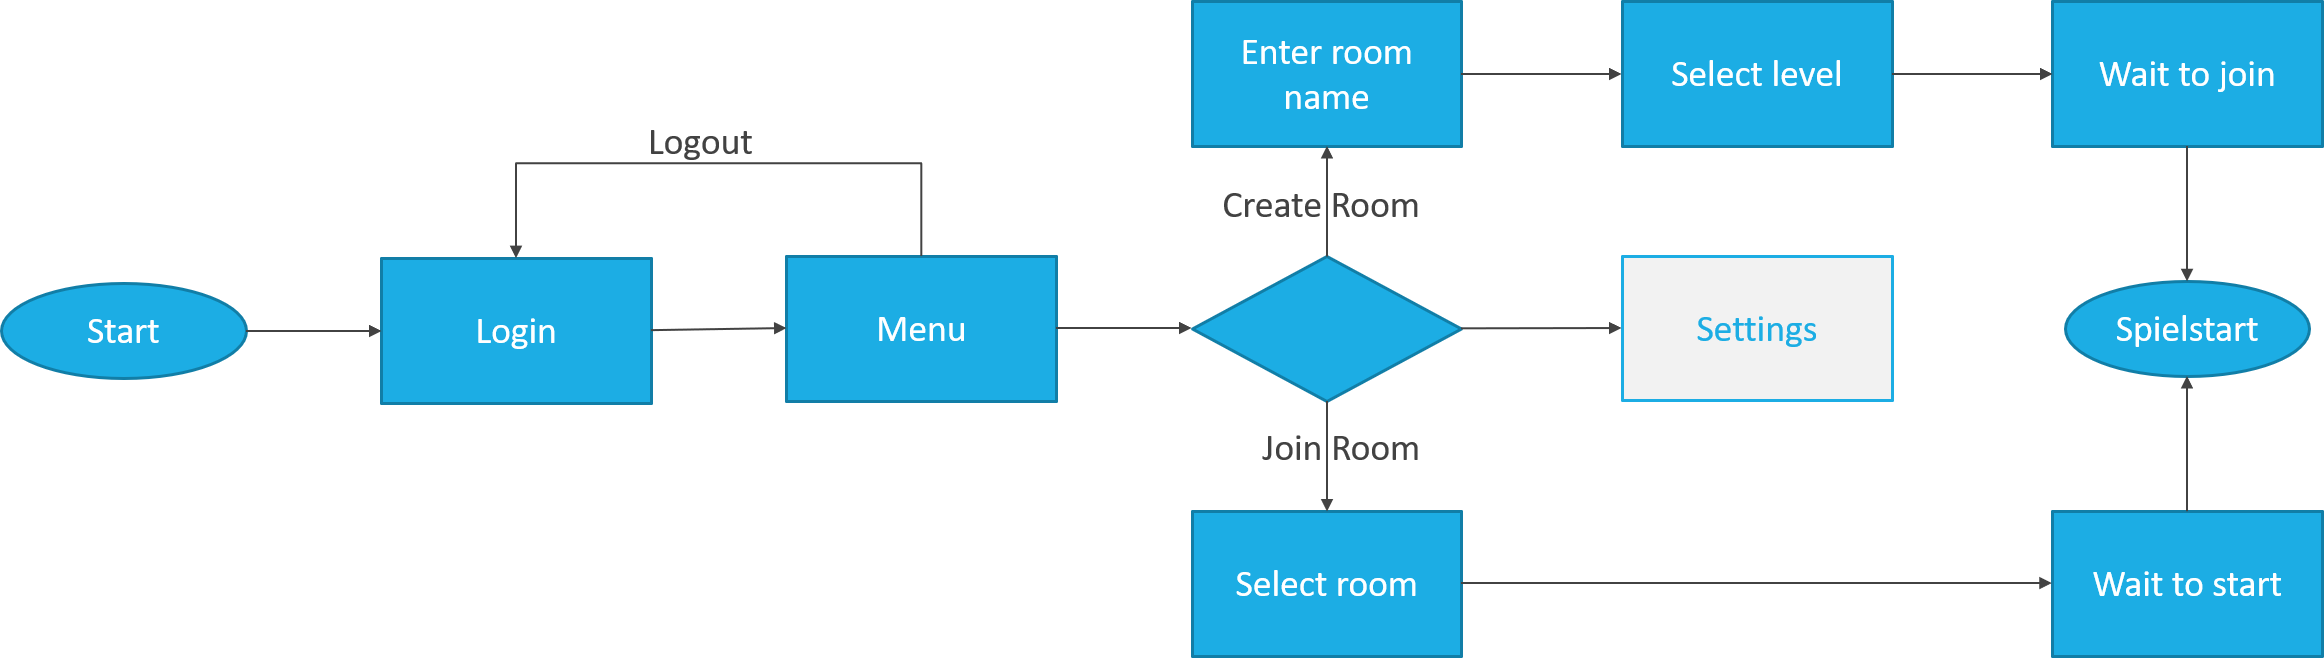
\includegraphics[width=\linewidth]{img/konzeption/Spielablauf2}
      \caption{Menüauswahl}
      \label{fig:konzeption:layout:menu}
    \end{center}
\end{figure}

Neben dem Erstellen bzw. Beitreten eines Raums kann man im Hauptmenü zusätzlich die Musiklautstärke verändern. Dabei kann die Hintergrundmusik, die In-Game-Geräusche und die Klick-Laustärke des Button-Feedbacks eingestellt werden.
\chapter{Realisierung}
\label{cha:realisierung}
In diesem Kapitel werden zunächst die Technologien besprochen, die für die Umsetzung nötig waren. Anschließend wird ausgeführt wie das Konzept schlussendlich umgesetzt wurde. Dabei wird auch das Design besprochen und auf Probleme bei der Umsetzung eingangen.

% Abschnitt: Technologien
\section{Technologien}
\label{sec:grundlagen:technologien}
Dieser Abschnitt dient dazu die genutzten Technologien kurz vorzustellen und eventuell auf Vor- und Nachteile sowie auf Besonderheiten einzugehen.

\subsection{Unity}
\label{subsec:realisierung:technologien:unity}
Unity ist eine Game-Engine der Firma \textit{Unity Technologies}. Die Entwicklungsumgebung der Game-Engine unterstützt mit integrierten Tools für Animation, Partikel-Systemen, Audio-Mixing und Tilemaps den gesamten Arbeitsablauf zum Erstellen von Spielen \cite{unity_mobile}. Unity erlaub dabei das Entwickln von Spielen auf die meisten Plattformen (Windows, Android, iOS, XBox, uvm.) und unterstützt dabei sowohl 2D-, als auch 3D-Spiele.

Im Folgendem werden die Vorteile, als auch die Nachteile der Spieleentwicklung mit Unity erläutert. Im Anschluss werden einige der Funktionen von Unity vorgestellt.
\subsubsection*{Vorteile}
\begin{itemize}
    \item Die von Unity verwendete Programmiersprache ist C\#, welche sehr ähnlich zu Java ist. Java als Programmiersprache ist uns (dem Team) gut geläufig, wodurch wir uns die Einarbeitungszeit in eine Programmiersprache ersparten.
    \item Unity unterstützt, die von uns vorgesehene Levelgestaltung, mit \textit{Tilemaps}. Damit wird das Bauen von Levelstrukturen und Hindernissen einfacher und schneller.
    \item Unity bietet durch seinen Asset-Store eine Großzahl an Vorlagen von jedlichen Spielfiguren, Plugins und weiteren vordefienierten Spielfunktionen (teils kostenpflichtig).
    \item Unity besitzt viele vordefinierte Funktionen, die dem Entwickler die Arbeit erheblich vereinfachen. Zum Beispiel können die im Spiel verwendete \textit{Physics} einfach konfiguriert werden und müssen nicht extra entwickelt werden.
    \item Das Builden der Anwendung auf Android (die Zielplattform) ist sehr schnell und unkompliziert. Allgemein besitzt Unity und Android eine gute Kompatibilität.
\end{itemize}

\subsubsection*{Nachteile}
\begin{itemize}
    \item Da für jedes selbst entwickelte Skript eine eigene Datei erstellt werden muss und Unity sehr viele Funktionen bereits implementiert hat, wird die Entwicklungsumgebung schnell unübersichtlich. Das erschwert das Arbeiten und verlangsamt den Arbeitsprozess.
    \item Unity ist eine (für uns) eine komlett neue Arbeitsumgebung. Die Levelgestaltung im Editor und unterschiedlichen Funktionen, die mit Unity einhergehen sind ungewohnt.
    \item Das Arbeiten im Team erfordert die Einbeziehung von Git, jedoch besitzt Unity keine gute Kompatibilität mit Git. Es treten nach dem Mergen oft Probleme auf und erschweren ein schnelles Entwickeln der Anwendung.
\end{itemize}

Unity ist eine Entwicklungsumgebung für Spiele mit geringer Einarbeitungszeit. Unity bietet mit seinen Funktionen die optimale Programmierumgebung um ein 2D-Jump 'n' Run-Muliplayer-Spiel zu erstellen. Einige der Funktionen werden im Folgenden vorgestellt.

\begin{description}
    \item[GameObjects] \hfill \\* Ein GameObject ist die Basisklasse für alle Entitäten einer Unity-Szene.
    \item[Components] \hfill \\* Eine Component ist eine Basisklasse für alles was mit GameObject verbunden ist.
    \item[Collider] \hfill \\* Collider sind in Unity dafür zuständig zu erkenn ob sich zwei Gameobjects berühren. Dadurch kann festgestellt werden ob der Spieler zum Beispiel auf der Spielfläche sich befindet oder ein Power-Up eingesammelt hat.
    \item[RayCasting] \hfill \\*
        RayCasting prüft wie ein Collider auf eine Kollision zwischen zwei Objekten. Der Vorteil ist allerdings das auch die Richtung der Kollision (oben, unten, rechts, links) bestimmt werden kann. Zudem kann man auch erkennen, wenn die Objekte kurz vor einer Kollision stehen, das ist insbesondere für den Walljump äußerst praktisch.
    \item[Tilemap] \hfill \\* Mit der Tilemap können schnell 2D-Ebenen erstellt werden. Tilemaps bestehen aus einem Gitter. Die verschiedenen Felder des Gitters können mit \textit{Tiles} gefüllt werden. Diese Tiles bilden die Spieloberfläche auf der der Spieler sich bewegen kann. Sind verschiedene Tiles verfügbar können schnell und einfach neue Level ganz einfach gezeichnet werden. \\ 
        Bei der Gestaltung von eigenen Tiles ist besonders wichtig, dass die Tiles zueinander passen, also bei einer Anordnung in einer horizontalen Reihe sollten die Tiles rechts und links ineinander übergehen. Hier ein Beispiel für solche Tiles: 
        \begin{figure}[H]
            \begin{center}
              
\includegraphics{img/realisierung/tile1.png}
              
\includegraphics{img/realisierung/tile2.png}
              
\includegraphics{img/realisierung/tile3.png}
              \label{fig:realisierung:realisierung:tiles}
            \end{center}
        \end{figure}
        
    \item[Prefabs] \hfill \\* Werden GameObjects mehrfach benötigt und ändern sich in ihrem Verhalten und Aussehen nicht, können Prefabs verwendet werden. Anstatt eine GameObject zu duplizieren und jedes Duplikat bei einer Änderung individuell zu ändern, haben Prefabs den Vorteil die vorgenommene Änderung auf alle Prefabs dieser Art zu übernehmen.
    \item[Inspector] \hfill \\* Projekte im Unity Editor bestehen aus GameObjects die Skripte, Sounds, usw. enthalten. Der Inspector zeigt detaillierte Informationen über jedes Component des ausgewählten GameObjects und erlaubt es dem Entwickler die Daten zu verändern.
    \item[Asset Store] \hfill \\* Der Asset Store ist wie der Nameschon sagt ein Store der viele Assets anbietet, die Entwickler dabei unterstützen ein Spiel zu entwickeln.
\end{description}

% TODO Code-Snippet aus Vortrag

\subsection{Photon}
\label{subsec:realisierung:technologien:photon}
Um Mulitplayer zu ermöglichen wird Photon verwendet. Photon verwaltet gemeinsame Sitzungen (Räume) von Spielern und ermöglicht es so, Nachrichten und Daten zwischen den verbunden Spielern plattformübergreifend in Echtzeit zu synchronisieren \cite{photon}.

Mit Photon kann man die neben den netzwerkrelevanten Daten auch die Position und Spielerinformationen unter den Spielern teilen. Dadurch können die jewiligen Endgeräte miteinander kommunizieren und ein gemeinsames Spielen ermöglichen. Dazu stellt Photon eine Vielzahl an Methoden zur Verfügung, die es dem Entwickler ermöglicht die Verbindung zwischen den Spielern aufzubauen, Räume zu erstellen und Spieldaten auszutauschen.

Eine nützliche Funktion Photons in der Spieleentwicklung sind \textit{Remote Procedure Calls} (RPC), die es ermöglichen Methoden in anderen Adressräumen aufzurufen. Dadurch können die Spieler untereinander Methoden aufrufen und direkt miteinander kommunizieren.

\subsection{Weitere Frameworks}
\label{subsec:realisierung:technologien:frameworks}
Für das An- und Abmelden von Spieleraccount wird eine \textit{Java REST Server} erstellt, der die Nutzer verwaltet. Dabei werden mit der Registrierung Nutzer erstellt und bei der Anmeldung überprüft, ob die jeweiligen Nutzer vorhanden sind und ob die eingegeben Nutzerdaten bei der Anmeldung korrekt sind. Zusätzlich übernimmt der Server die Funktion, die Level nach dem Beendigen des vorherigen Level freizuschalten. Der Server speichert somit neben den Nutzerdaten, die Levelfreigabe der jeweiligen Nutzer. Der Server verwendet dabei eine PostgresSQL-Datenbank.

\subsection{Architektur}
\label{subsec:realisierung:technologien:architektur}
% Zusammenspiel von Photon, Unity und Server
Wie Photon und der Java REST Server mit Unity kommunizieren, zeigt Abbildung \ref{fig:realisierung:technologien:architektur}. Nach dem Start der Unity-Anwendung ist der REST-Server für die Anmeldung und die Levelauswahl zuständig. Anschließend verwaltet Photon die verschiedenen Räume und das Spiel an sich.

\begin{figure}[H]
    \begin{center}
      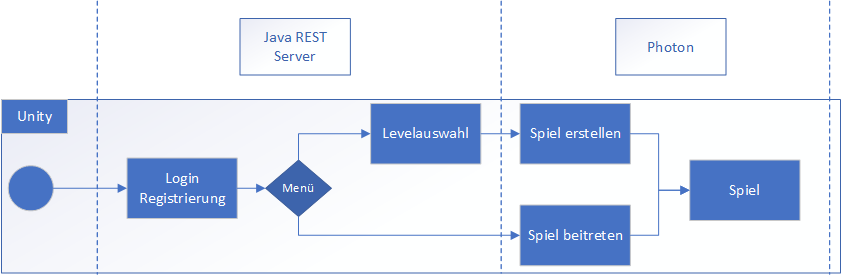
\includegraphics[width=\linewidth]{img/realisierung/Architektur}
      \caption{Architektur}
      \label{fig:realisierung:technologien:architektur}
    \end{center}
\end{figure}

%\subsection{Unity \& Mobile Applications}
%\label{subsec:implementierung:technologien:mobile}
% ich weiß nicht was da rein soll^^ TODO

\section{Umsetzung}
\label{sec:grundlagen:umsetzung}
Nachdem das Spielkonzept und die Programmierumgebung vorgestellt wurden, wird nun die Umsetzung des Spiels vorgestellt. Dabei werden wichtige Codebeispiele und die Funktionen verschiedener Spielobjekte vorgestellt. Zusätzlich wird auf das Menü, der Spielablauf und die Levelgestaltung zum Erzwingen von Teamplay eingegangen.

\subsection{Codebeispiele}
\label{subsec:implementierung:umsetzung:codebeispiele}
Um neben den verschiedenen UI-Elementen und den Leveldesigns auch die erstellte Funktionalität vorzustellen, werden kurze Codebeispiele gezeigt. Als Beispiel wird wie in Kapitel \ref{subsec:realisierung:technologien:photon} die RPC-Aufrufe kurz dargestellt und erläutert. Das Codebeispiel \ref{lst:implementierung:umsetzung:codebeispiele1} zeigt wie nach dem Start des Skripts die Methode \texttt{StartGameRPC} mit Hilfe eines RPC-Aufruf aufgerufen wird. Der Aufruf richtet sich dabei an alle Spieler, die sich in dem Raum befinden (vgl. \texttt{PhotonTargets.All}). Anschließend können weiter Parameter übergeben werden (hier der Name des zu startende Levels).

Die Methoden die über einen RPC-Aufruf erreichbar gemacht werden sollen, werden mit \texttt{PunRPC} gekennzeichnet.

\begin{lstlisting}[caption={RPC-Aufrufe}, label=lst:implementierung:umsetzung:codebeispiele1]
public class PhotonExample : PunBehaviour {

    public void Start() {        
        photonView.RPC("StartGameRPC",PhotonTargets.All,"lvl01");    
    }
    
    [PunRPC]    
    public void StartGameRPC(string sceneName) {        
        NetworkManager.Reference.StartGame(sceneName);    
    }
}
\end{lstlisting}

\subsection{Szenen und Spielobjekte}
\label{subsec:implementierung:umsetzung:realisierung}
In diesem Kapitel werden die verschiedenen Szenen und Spielobjekte vorgestellt. Dabei wird der Aufbau der Level und die Funktionsweise der Spielobjekte aufgezeigt.

\subsubsection{Menü}
\label{subsubsec:implementierung:umsetzung:realisierung:menu}

Das Menü mit dem Login und der Spielerstellung ist der Einstiegspunkt des Spiels. Der gesamte Menü-Dialog ist eine Szene, die durch aus- und einblenden von UI-Elementen das Erstellen des Spiels und das Verändern der Einstellungen ermöglicht. Der Hintergrund der Menü-Szene verwendet \textit{Parallax-Scrolling} um die ansonsten statische Spielumgebung dynamischer zu gestalten. Durch Parallax-Scrolling bewegt sich der Hintergrund stetig von rechts nach links. Zum Starten des Hauptmenüs muss der Nutzer den Usernamen und das Passwort eingeben. Er muss sich dafür registrieren und anschließend anmelden. 

Damit der Input für Nutzername und Passwort valide ist, wird überprüft, ob überhaupt etwas eingetragen wurde und ob der Input zwischen 1 und 32 Zeichen liegt. Ansonsten erscheint ein Hinweis der den Nutzer darauf hinweist.

\begin{figure}[H]
    \begin{center}
      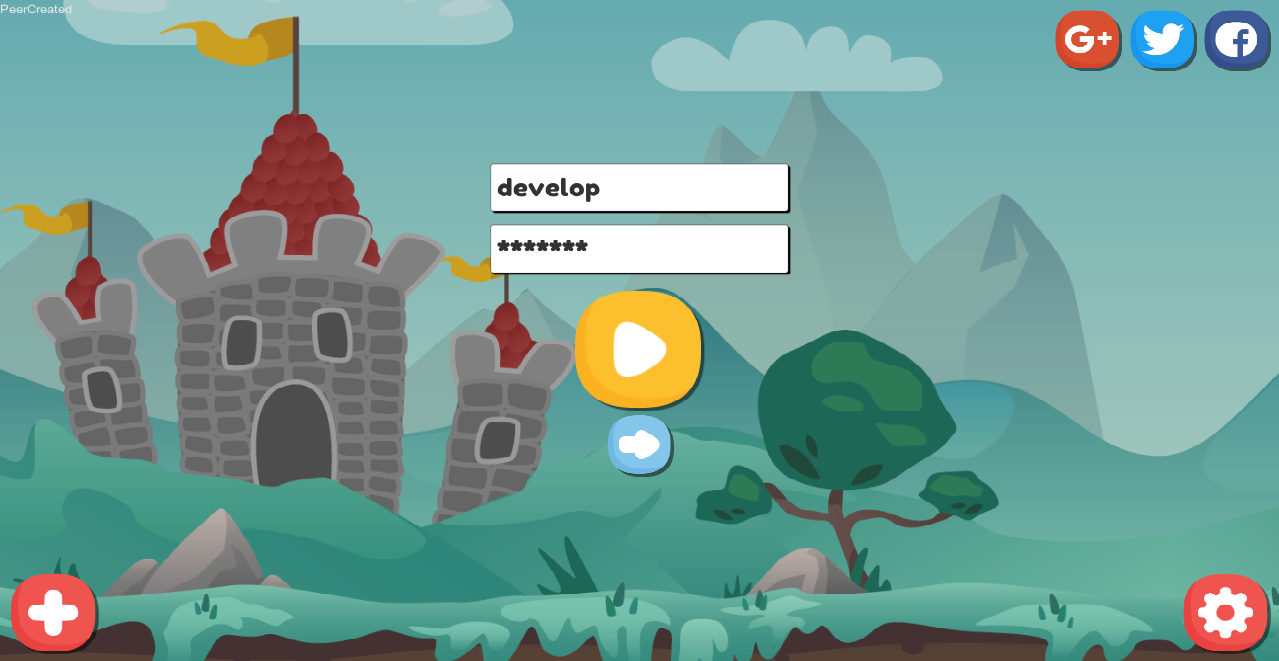
\includegraphics[width=\linewidth]{img/realisierung/Login}
      \caption{Login und Registrierung}
      \label{fig:realisierung:realisierung:login}
    \end{center}
\end{figure}

Im Hauptmenü entscheidet der Spieler, ob er ein Spiel erstellt oder einem bereits erstelltem Spiel beitritt. Zusätzlich kann der Nutzer seine Einstellungen ändern und sich Ausloggen.

\begin{figure}[H]
    \begin{center}
      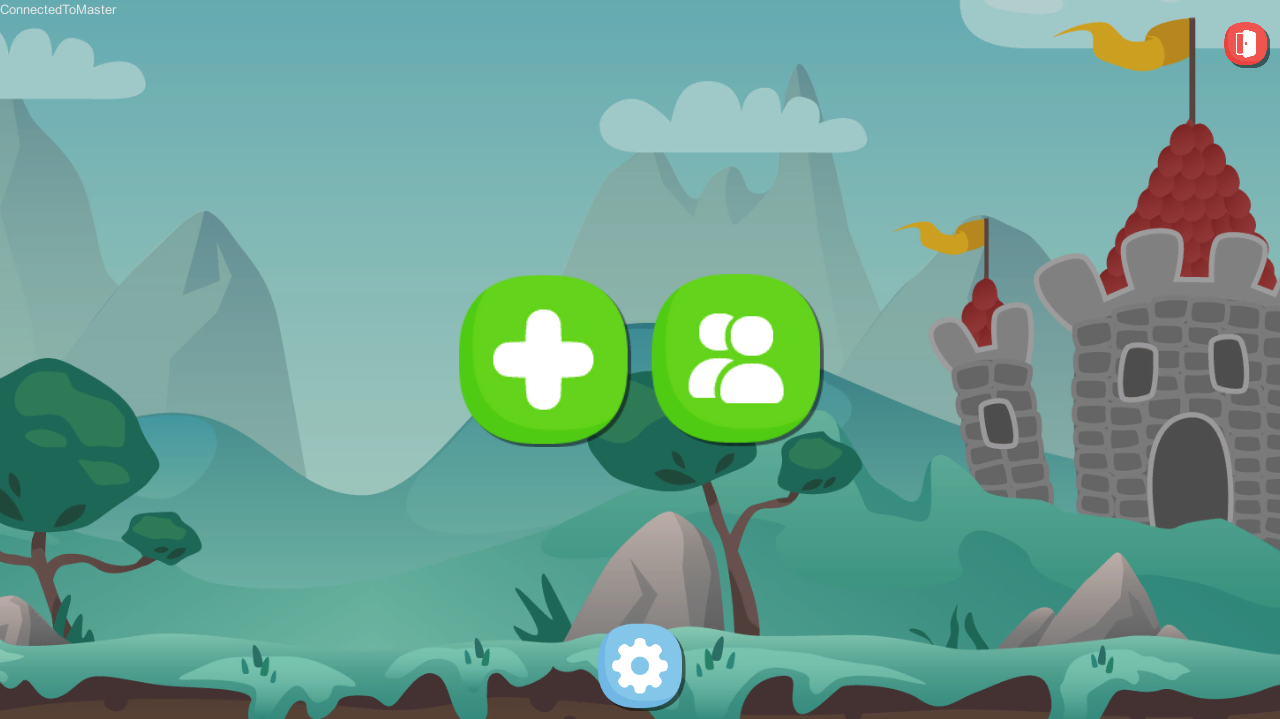
\includegraphics[width=\linewidth]{img/realisierung/menu}
      \caption{Hauptmenü}
      \label{fig:realisierung:realisierung:hauptmenu}
    \end{center}
\end{figure}

Das Spiel bietet dem Spieler die Möglichkeit die Lautstärke zu ändern. Dabei können drei verschiedene Lautstärken verändert werden. Zum einen kann die Hintergrundmusiklautstärke der jeweiligen Szene und zum anderen die In-Game-Geräsche (Springen, Schaden, Nutzen von Portalen) verändert werden. Die dritte Möglichkeit ist es das Audiofeedback nach einem Buttonklick zu variieren. Diese drei Audiomanager sind voneinander unabhängig und können so individuell verändert werden.

\begin{figure}[H]
    \begin{center}
      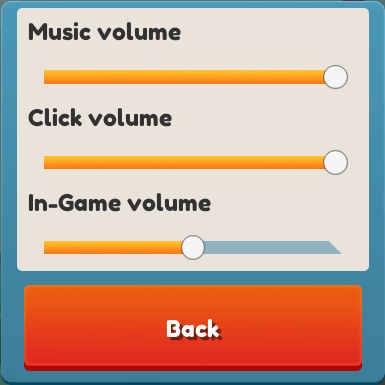
\includegraphics[width=.33\linewidth]{img/realisierung/settings}
      \caption{Lautstärkeneinstellungen}
      \label{fig:realisierung:realisierung:settings}
    \end{center}
\end{figure}

\subsubsection{Level}
\label{subsubsec:implementierung:umsetzung:realisierung:level}
Neben den Hintergrundbild sind es die Tiles, die dem jeweiligen Level das Thema verleihen. Da jedes Level sich mit einem eigenen Thema beschäftigen soll, wurden in jedem Level vier verschiedene Tiles verwendet (vgl. Abbildung \ref{fig:realisierung:realisierung:level:tiles}). Die Tiles bilden die Spieloberfläche auf der sich die Spieler bewegen können. 

\begin{figure}[H]
    \begin{center}
      
\includegraphics[width=.5\linewidth]{img/realisierung/assets/tiles_2}
      \caption{Tiles}
      \label{fig:realisierung:realisierung:level:tiles}
    \end{center}
\end{figure}

Plattformen sind wie in den meisten Jump 'n' Run-Spielen dafür zuständig die Spieler zu transportieren. Sie passen vom Thema her zu den Tiles und folgen einem vorgegebenen Pfad. 

\begin{figure}[H]
    \begin{center}
      
\includegraphics[width=.1\linewidth]{img/realisierung/assets/plattform}
      \caption{Plattform}
      \label{fig:realisierung:realisierung:level:plattform}
    \end{center}
\end{figure}

Um das Level abschließen zu können müssen die Spieler zwei Schlüssel einsammeln. Je nach Schwierigkeit des jeweiligen Levels können sie versteckt oder einfach zugänglich sein. Erst wenn beide Schlüssel (egal von welchem Spieler) eingesammelt sind, kann das Spiel beendet werden. Das Ziel des Spiels ist es eine Truhe zu erreichen. 

Damit das Level dynamischer und komplexer gestaltet wird, werden verschiedene Spielobjekte die Spieler während des Spielverlaufs unterstützen oder schaden. Im Folgenden werden diese Spielobjekte vorgestellt.

\subsubsection{Spielobjekte}
\label{subsubsec:implementierung:umsetzung:realisierung:spielobjekte}
Alle Spielobjekte haben direkten Einfluss auf das Spiel (ausgenommen die Münze). Sie können den Spielern schaden, ihr Leben erneuern oder sie transportieren. 

In Abbildung \ref{fig:keyandchest} wird der Schlüssel und die Truhe dargestellt, welche im Laufe des Spiels erreicht werden müssen, da ansonsten das Level nicht beendet werden kann. Die Spieler müssen beide Schlüssel einsammeln, damit sich die Truhe öffnet und das Level abschließt.

\begin{figure}[H]
    \centering
    \begin{subfigure}[H]{0.15\textwidth}
        
\includegraphics[width=\textwidth]{img/realisierung/assets/chest}
        \caption{Truhe}
        \label{fig:truhe}
    \end{subfigure}
    \qquad
    \begin{subfigure}[H]{0.15\textwidth}
        
\includegraphics[width=\textwidth]{img/realisierung/assets/key}
        \caption{Schlüssel}
        \label{fig:schluessel}
    \end{subfigure}
    \caption{Levelrelevante Spielobjekte}
    \label{fig:keyandchest}
\end{figure}

Das Level stellt auch Hindernisse für die Spieler. Durch bewegliche und statische Hindernisse wird das Spiel schwieriger. Abbildung \ref{fig:mace} zeig ein \textit{Mace}, dass einem vorgegebenen Pfad folgt. Statische Hindernisse in Form von \textit{Spikes} werden in Abbildung \ref{fig:spike} dargestellt. Der Spieler verliert bei Kontakt mit diesen Hindernissen Leben. Berührt er ein Hindernis zu oft oder zu lange stirbt der jeweilige Spieler und das Level muss von beiden Spielern neu gestartet werden.

\begin{figure}[H]
    \centering
    \begin{subfigure}[H]{0.15\textwidth}
        
\includegraphics[width=\textwidth]{img/realisierung/assets/mace}
        \caption{Mace}
        \label{fig:mace}
    \end{subfigure}
    \qquad
    \begin{subfigure}[H]{0.15\textwidth}
        
\includegraphics[width=\textwidth]{img/realisierung/assets/spike}
        \caption{Spike}
        \label{fig:spike}
    \end{subfigure}
    \caption{Hindernisse im Spiel}
    \label{fig:maceandspike}
\end{figure}

Sollte ein Spieler leben verloren haben, kann er durch das Einsammeln eines Power-Ups geheilt werden (vgl. Abbildung \ref{fig:eat}). Dieses Power-Up heilt ein Teil des verlorenen Lebens. 
Levelübergreifend kann der Spieler Münzen sammeln. Die Münzen haben eine kompetitive Funktion. Spieler können sich daran messen, wer eine größere Anzahl an Münzen besitzt. Eine Münze wird in Abbildung \ref{fig:coin} dargestellt.

\begin{figure}[H]
    \centering
    \begin{subfigure}[H]{0.15\textwidth}
        
\includegraphics[width=\textwidth]{img/realisierung/assets/eat}
        \caption{Power-Up}
        \label{fig:eat}
    \end{subfigure}
    \qquad
    \begin{subfigure}[H]{0.15\textwidth}
        
\includegraphics[width=\textwidth]{img/realisierung/assets/coin}
        \caption{Münze}
        \label{fig:coin}
    \end{subfigure}
    \caption{Power-Ups im Spiel}
    \label{fig:eatandcoin}
\end{figure}

Das Spielkonzept der Zusammenarbeit der Spieler wurde durch das Verwenden von Portalen und Barrieren ermöglicht. Barrieren sind nur für den Spieler durchlässig, der die selbe Farbe wie die Barriere besitzt (vgl. Abbildung \ref{fig:barriere}). Der andere Spieler kann diese Barriere nicht durchqueren. Dadurch müssen Spieler verschiedene Wege gehen oder nur ein bestimmter Spieler kann ein bestimmtes Spielobjekt (Schlüssel, Power-Up) erreichen.

Um das Spiel noch etwas dynamischer zu gestalten, können die Spieler die in Abbildung \ref{fig:portal} dargestellten Portale benutzen. Jedes Portal hängt mit einem weiteren Portal zusammen, zu dem der Spieler beim Betreten des ersten Portal teleportiert wird und umgekehrt. Dadurch können Spielbereiche erreicht werden, die der Spieler ohne das Verwenden von Portalen nicht erreichen kann.

\begin{figure}[H]
    \centering
    \begin{subfigure}[H]{0.10\textwidth}
        
\includegraphics[width=\textwidth]{img/realisierung/assets/barriere}
        \caption{Barriere}
        \label{fig:barriere}
    \end{subfigure}
    \qquad
    \begin{subfigure}[H]{0.15\textwidth}
        
\includegraphics[width=\textwidth]{img/realisierung/assets/portal}
        \caption{Portal}
        \label{fig:portal}
    \end{subfigure}
    \caption{Spielerweiternde Spielobjekte}
    \label{fig:barriereandportal}
\end{figure}

\newpage
\section{Probleme}
\label{sec:implementierung:probleme}
% Design von Assets -> Kostenlose genommen, da aufwändig
\begin{description}
    \item[Git] \hfill \\* Wie in Kapitel \ref{subsec:realisierung:technologien:unity} bereits erwähnt, ist die Kompatibilität von Unity und Git verbesserungsfähig. Bei der Entwicklung sind oft unvorhergesehene Refernzfehler aufgetreten, was das Spiel unspielbar machte und einige Zeit zum Aussbessern benötigte.
    \item[Assets] \hfill \\* Das Erstellen von UI-Elementen ist sehr aufwändig. Zusätzlich benötigt man für ein visuell ansprechendes UI-Element eine gewisse künstlerische Begabung, die nicht immer vorhanden ist. Sollen die verschiedenen UI-Elemente Animiert sein, muss jeder Frame extra gemalt werden. Diese bedeutet einen großen Aufwand mit unbefriedigenden Resultaten. Daher wurde für die Entwicklung dieser Anwendung vorgefertigte Assets verwendet.
    \item[Musik/Sounds] \hfill \\* Ähnlich wie bei den Assets sollten ursprünglich eigene Soundeffekte und Musik verwendet werden. Doch das Erstellen gestaltete sich als kompizierter und aufwändiger als gedacht. Daher haben wir auch in diesem Fall auf eine vorgefertigte und kostenlose Variante zurückgegriffen.
\end{description}






























\chapter{Zusammenfassung \& Ausblick}
\label{cha:zusammenfassungAusblick}
In diesem letzten Kapitel wird die Arbeit nochmal zusammengefasst um anschließend einen Ausblick für die Zukunft zu geben.

% Abschnitt: Zusammenfassung
\section{Zusammenfassung}
\label{sec:grundlagen:zusammenfassung}
Da Unity als Engine schon viele vordefinierte Funktionen anbietet, darunter zum Beispiel die Collision Detection, ist das Arbeiten zunächst ungewohnt im Gegensatz zur Arbeit mit einer Entwicklungsumgebung wie Android Studio. Ein Grund dafür ist, das ein großer Anteil nicht über Programmcode, sondern über die GUI Oberfläche die Unity zur Verfügung stellt realisiert wird. Der Inspector des Editors lässt die Componenten der Gameobjects mit den jeweiligen Attributen schnell verändern. Dadurch ist das fertige Spiel sehr wandlungsfähig und kann nach belieben im Detail angepasst werden. 

Nach dem Fertigstellen der App kann durch die gute Kompatibilität von Unity mit sehr vielen Plattformen das Spiel nicht nur auf Android, sondern auf weiteren Plattformen verwendet werden. Dadurch, und durch die Verwendung von Phton, wird unsere Abyss-Anwendung zu einem \textit{Crossplatform game}.

Das Verwenden von eigenen UI-Elementen sollte man als Design-Anfänger oursourcen, da das Erstellen von Bilder, die visuell ansprechend sein sollen, eine künsterische Ader erfordert. Das gleiche gilt für die Erstellung von eigenen Soundeffekten und Hintergrundmusik. Man kann durch die Verwendung von eigenen Materialien das Spiel sehr individualisieren, doch ist der Aufwand, der hinter dieser Arbeit steckt, nicht zu unterschätzen. 

Das Projektmanagement der Unity-Anwendung ist mit Git fehleranfällig. Erstellt man jedoch für jedes Problem einen eigenen Branch können die enstehenden Probleme minimal gehalten werden.

% Abschnitt: Ausblick
\section{Ausblick}
\label{sec:grundlagen:ausblick}
Nachdem das Grundgerüst des Spiels mit den selbstentworfenen Funktionen und Assets erstellt wurde, ist das Spiel schnell und simpel erweiterbar. Durch das Verwenden von Prefabs und den vorhandenen Tilemaps können in kürze Spielflächen erstellt und Hindernisse hinzugefügt werden. Um neue Spielobjekte zu erstellen, können die vorhandenen Skripte angefügt und durch neue, aber simple Skripte erweitert werden. Dadurch kann das Spiel nicht nur an Leveln, sondern auch an Spielkomplexität wachsen.

% Bibliograhpy
\bibliographystyle{splncs}
\begingroup
\interlinepenalty 10000
\sloppy
\bibliography{literature}
\endgroup

% anhänge
\appendix

\backmatter			% abtrennung für verzeichnisse

% hier die verzeichnisse
\listoffigures

\end{document}
